% Created by tikzDevice version 0.12.3.1 on 2022-11-28 20:42:03
% !TEX encoding = UTF-8 Unicode
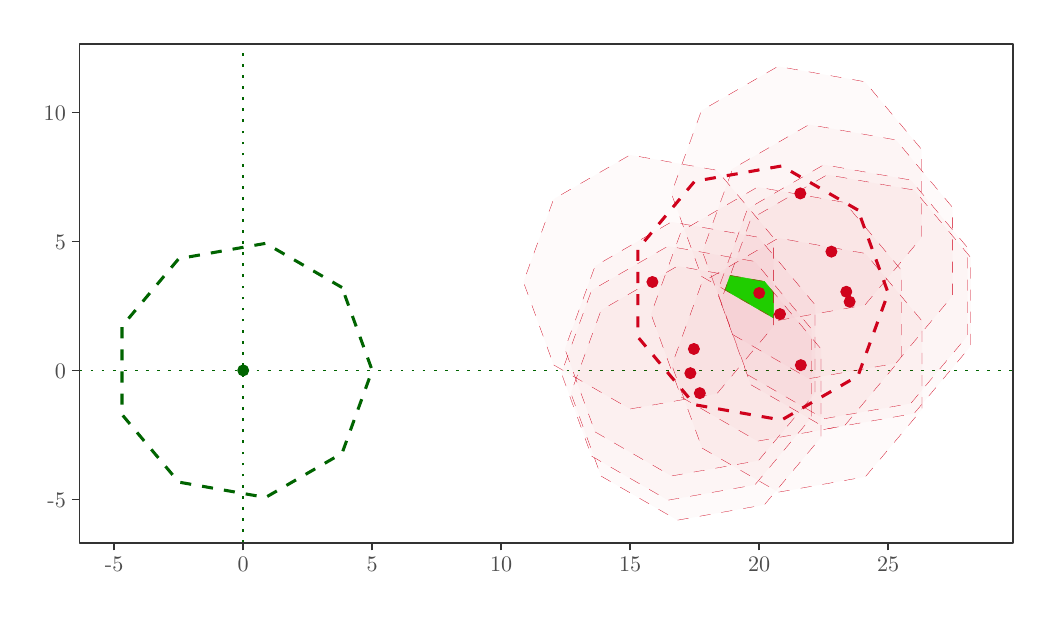
\begin{tikzpicture}[x=1pt,y=1pt]
\definecolor{fillColor}{RGB}{255,255,255}
\begin{scope}
\definecolor{drawColor}{RGB}{255,255,255}
\definecolor{fillColor}{RGB}{255,255,255}

\path[draw=drawColor,line width= 0.6pt,line join=round,line cap=round,fill=fillColor] (  0.00,187.39) rectangle (361.35,390.77);
\end{scope}
\begin{scope}
\definecolor{fillColor}{RGB}{255,255,255}

\path[fill=fillColor] ( 18.45,204.90) rectangle (355.85,385.27);
\definecolor{drawColor}{RGB}{0,100,0}

\path[draw=drawColor,line width= 1.1pt,dash pattern=on 4pt off 4pt ,line join=round,even odd rule]
	(113.29,297.18) --
	( 85.68,313.13) --
	( 54.28,307.59) --
	( 33.78,283.17) --
	( 33.78,251.28) --
	( 54.28,226.86) --
	( 85.68,221.32) --
	(113.29,237.26) --
	(124.19,267.22) --
	(113.29,297.18) --
	cycle;
\definecolor{fillColor}{RGB}{0,100,0}

\path[draw=drawColor,line width= 0.4pt,line join=round,fill=fillColor] ( 77.58,267.22) circle (  1.96);
\definecolor{drawColor}{RGB}{208,2,28}

\path[draw=drawColor,line width= 1.1pt,dash pattern=on 4pt off 4pt ,line join=round,even odd rule]
	(299.73,325.15) --
	(272.12,341.09) --
	(240.72,335.56) --
	(220.23,311.13) --
	(220.23,279.25) --
	(240.72,254.82) --
	(272.12,249.29) --
	(299.73,265.23) --
	(310.64,295.19) --
	(299.73,325.15) --
	cycle;
\definecolor{drawColor}{RGB}{0,255,0}
\definecolor{fillColor}{RGB}{0,255,0}

\path[draw=drawColor,line width= 0.2pt,line join=round,fill=fillColor,even odd rule]
	(265.89,299.37) --
	(269.25,295.36) --
	(269.25,286.16) --
	(251.67,296.31) --
	(253.57,301.54) --
	(265.89,299.37) --
	cycle;
\definecolor{drawColor}{RGB}{0,100,0}

\path[draw=drawColor,line width= 0.6pt,dash pattern=on 1pt off 3pt ,line join=round] ( 18.45,267.22) -- (355.85,267.22);

\path[draw=drawColor,line width= 0.6pt,dash pattern=on 1pt off 3pt ,line join=round] ( 77.58,204.90) -- ( 77.58,385.27);
\definecolor{drawColor}{RGB}{208,2,28}
\definecolor{fillColor}{RGB}{208,2,28}

\path[draw=drawColor,line width= 0.4pt,line join=round,fill=fillColor] (264.03,295.19) circle (  1.96);

\path[draw=drawColor,line width= 0.4pt,line join=round,fill=fillColor] (296.71,292.02) circle (  1.96);

\path[draw=drawColor,line width= 0.4pt,line join=round,fill=fillColor] (242.58,259.00) circle (  1.96);

\path[draw=drawColor,line width= 0.4pt,line join=round,fill=fillColor] (240.43,274.97) circle (  1.96);

\path[draw=drawColor,line width= 0.4pt,line join=round,fill=fillColor] (225.45,299.17) circle (  1.96);

\path[draw=drawColor,line width= 0.4pt,line join=round,fill=fillColor] (279.08,269.12) circle (  1.96);

\path[draw=drawColor,line width= 0.4pt,line join=round,fill=fillColor] (278.89,331.17) circle (  1.96);

\path[draw=drawColor,line width= 0.4pt,line join=round,fill=fillColor] (239.16,266.22) circle (  1.96);

\path[draw=drawColor,line width= 0.4pt,line join=round,fill=fillColor] (271.55,287.56) circle (  1.96);

\path[draw=drawColor,line width= 0.4pt,line join=round,fill=fillColor] (295.51,295.64) circle (  1.96);

\path[draw=drawColor,line width= 0.4pt,line join=round,fill=fillColor] (290.13,310.14) circle (  1.96);
\definecolor{fillColor}{RGB}{208,2,28}

\path[draw=drawColor,line width= 0.1pt,dash pattern=on 4pt off 4pt ,line join=round,fill=fillColor,fill opacity=0.02,even odd rule]
	(261.01,262.05) --
	(288.62,246.11) --
	(320.02,251.65) --
	(340.51,276.07) --
	(340.51,307.96) --
	(320.02,332.38) --
	(288.62,337.92) --
	(261.01,321.98) --
	(250.10,292.02) --
	(261.01,262.05) --
	cycle;

\path[draw=drawColor,line width= 0.1pt,dash pattern=on 4pt off 4pt ,line join=round,fill=fillColor,fill opacity=0.02,even odd rule]
	(206.88,229.04) --
	(234.49,213.10) --
	(265.89,218.64) --
	(286.38,243.06) --
	(286.38,274.95) --
	(265.89,299.37) --
	(234.49,304.91) --
	(206.88,288.97) --
	(195.97,259.00) --
	(206.88,229.04) --
	cycle;

\path[draw=drawColor,line width= 0.1pt,dash pattern=on 4pt off 4pt ,line join=round,fill=fillColor,fill opacity=0.02,even odd rule]
	(204.72,245.01) --
	(232.34,229.07) --
	(263.74,234.61) --
	(284.23,259.03) --
	(284.23,290.92) --
	(263.74,315.34) --
	(232.34,320.88) --
	(204.72,304.93) --
	(193.82,274.97) --
	(204.72,245.01) --
	cycle;

\path[draw=drawColor,line width= 0.1pt,dash pattern=on 4pt off 4pt ,line join=round,fill=fillColor,fill opacity=0.02,even odd rule]
	(189.75,269.21) --
	(217.36,253.27) --
	(248.76,258.81) --
	(269.25,283.23) --
	(269.25,315.11) --
	(248.76,339.54) --
	(217.36,345.07) --
	(189.75,329.13) --
	(178.84,299.17) --
	(189.75,269.21) --
	cycle;

\path[draw=drawColor,line width= 0.1pt,dash pattern=on 4pt off 4pt ,line join=round,fill=fillColor,fill opacity=0.02,even odd rule]
	(243.37,239.16) --
	(270.98,223.22) --
	(302.38,228.76) --
	(322.88,253.18) --
	(322.88,285.07) --
	(302.38,309.49) --
	(270.98,315.03) --
	(243.37,299.08) --
	(232.47,269.12) --
	(243.37,239.16) --
	cycle;

\path[draw=drawColor,line width= 0.1pt,dash pattern=on 4pt off 4pt ,line join=round,fill=fillColor,fill opacity=0.02,even odd rule]
	(243.18,301.21) --
	(270.80,285.27) --
	(302.20,290.80) --
	(322.69,315.23) --
	(322.69,347.11) --
	(302.20,371.54) --
	(270.80,377.07) --
	(243.18,361.13) --
	(232.28,331.17) --
	(243.18,301.21) --
	cycle;

\path[draw=drawColor,line width= 0.1pt,dash pattern=on 4pt off 4pt ,line join=round,fill=fillColor,fill opacity=0.02,even odd rule]
	(203.46,236.26) --
	(231.07,220.32) --
	(262.47,225.85) --
	(282.96,250.28) --
	(282.96,282.16) --
	(262.47,306.58) --
	(231.07,312.12) --
	(203.46,296.18) --
	(192.55,266.22) --
	(203.46,236.26) --
	cycle;

\path[draw=drawColor,line width= 0.1pt,dash pattern=on 4pt off 4pt ,line join=round,fill=fillColor,fill opacity=0.02,even odd rule]
	(235.85,257.60) --
	(263.46,241.66) --
	(294.86,247.20) --
	(315.35,271.62) --
	(315.35,303.51) --
	(294.86,327.93) --
	(263.46,333.47) --
	(235.85,317.53) --
	(224.94,287.56) --
	(235.85,257.60) --
	cycle;

\path[draw=drawColor,line width= 0.1pt,dash pattern=on 4pt off 4pt ,line join=round,fill=fillColor,fill opacity=0.02,even odd rule]
	(259.80,265.68) --
	(287.41,249.74) --
	(318.81,255.28) --
	(339.31,279.70) --
	(339.31,311.59) --
	(318.81,336.01) --
	(287.41,341.55) --
	(259.80,325.60) --
	(248.90,295.64) --
	(259.80,265.68) --
	cycle;

\path[draw=drawColor,line width= 0.1pt,dash pattern=on 4pt off 4pt ,line join=round,fill=fillColor,fill opacity=0.02,even odd rule]
	(254.43,280.18) --
	(282.04,264.24) --
	(313.44,269.78) --
	(333.93,294.20) --
	(333.93,326.08) --
	(313.44,350.51) --
	(282.04,356.04) --
	(254.43,340.10) --
	(243.52,310.14) --
	(254.43,280.18) --
	cycle;
\definecolor{drawColor}{gray}{0.20}

\path[draw=drawColor,line width= 0.6pt,line join=round,line cap=round] ( 18.45,204.90) rectangle (355.85,385.27);
\end{scope}
\begin{scope}
\definecolor{drawColor}{gray}{0.30}

\node[text=drawColor,anchor=base east,inner sep=0pt, outer sep=0pt, scale=  0.80] at ( 13.50,217.86) { -5};

\node[text=drawColor,anchor=base east,inner sep=0pt, outer sep=0pt, scale=  0.80] at ( 13.50,264.47) {  0};

\node[text=drawColor,anchor=base east,inner sep=0pt, outer sep=0pt, scale=  0.80] at ( 13.50,311.08) {  5};

\node[text=drawColor,anchor=base east,inner sep=0pt, outer sep=0pt, scale=  0.80] at ( 13.50,357.69) { 10};
\end{scope}
\begin{scope}
\definecolor{drawColor}{gray}{0.20}

\path[draw=drawColor,line width= 0.6pt,line join=round] ( 15.70,220.61) --
	( 18.45,220.61);

\path[draw=drawColor,line width= 0.6pt,line join=round] ( 15.70,267.22) --
	( 18.45,267.22);

\path[draw=drawColor,line width= 0.6pt,line join=round] ( 15.70,313.83) --
	( 18.45,313.83);

\path[draw=drawColor,line width= 0.6pt,line join=round] ( 15.70,360.44) --
	( 18.45,360.44);
\end{scope}
\begin{scope}
\definecolor{drawColor}{gray}{0.20}

\path[draw=drawColor,line width= 0.6pt,line join=round] ( 30.97,202.15) --
	( 30.97,204.90);

\path[draw=drawColor,line width= 0.6pt,line join=round] ( 77.58,202.15) --
	( 77.58,204.90);

\path[draw=drawColor,line width= 0.6pt,line join=round] (124.19,202.15) --
	(124.19,204.90);

\path[draw=drawColor,line width= 0.6pt,line join=round] (170.81,202.15) --
	(170.81,204.90);

\path[draw=drawColor,line width= 0.6pt,line join=round] (217.42,202.15) --
	(217.42,204.90);

\path[draw=drawColor,line width= 0.6pt,line join=round] (264.03,202.15) --
	(264.03,204.90);

\path[draw=drawColor,line width= 0.6pt,line join=round] (310.64,202.15) --
	(310.64,204.90);
\end{scope}
\begin{scope}
\definecolor{drawColor}{gray}{0.30}

\node[text=drawColor,anchor=base,inner sep=0pt, outer sep=0pt, scale=  0.80] at ( 30.97,194.44) { -5};

\node[text=drawColor,anchor=base,inner sep=0pt, outer sep=0pt, scale=  0.80] at ( 77.58,194.44) {  0};

\node[text=drawColor,anchor=base,inner sep=0pt, outer sep=0pt, scale=  0.80] at (124.19,194.44) {  5};

\node[text=drawColor,anchor=base,inner sep=0pt, outer sep=0pt, scale=  0.80] at (170.81,194.44) { 10};

\node[text=drawColor,anchor=base,inner sep=0pt, outer sep=0pt, scale=  0.80] at (217.42,194.44) { 15};

\node[text=drawColor,anchor=base,inner sep=0pt, outer sep=0pt, scale=  0.80] at (264.03,194.44) { 20};

\node[text=drawColor,anchor=base,inner sep=0pt, outer sep=0pt, scale=  0.80] at (310.64,194.44) { 25};
\end{scope}
\end{tikzpicture}
